\chapter{\IfLanguageName{dutch}{Stand van zaken}{State of the art}}%
\label{ch:stand-van-zaken}

% Tip: Begin elk hoofdstuk met een paragraaf inleiding die beschrijft hoe
% dit hoofdstuk past binnen het geheel van de bachelorproef. Geef in het
% bijzonder aan wat de link is met het vorige en volgende hoofdstuk.

% Pas na deze inleidende paragraaf komt de eerste sectiehoofding.

In dit hoofdstuk zal de literatuurstudie besproken worden. Door deze literatuurstudie is het mogelijk om een beter inzicht te krijgen in de technologie en mogelijkheden voor de documentatie van Python projecten. 
Alsook hoe het toegepast kan worden met behulp van Large Language Modellen. Er
zal nadruk worden gelegd op bestaande literatuur en onderzoeken die verbonden
zijn met documentatie van Python projecten. In dit onderdeel zullen verschillende hoofdstukken worden aangekaart. 
Als eerste zal er duidelijk gemaakt worden wat er juist verstaan wordt met documentatie. 
Dan wordt er gekeken naar wat Large Language Modellen zijn, hoe deze werken en wat enkele bestaande modellen zijn.
Vervolgens wordt er gekeken naar bestaande documentatie tools.
Als laatste wordt er gekeken naar hoe Large Language Modellen gebruikt kunnen worden voor het genereren van documentatie.

\section{Wat is documentatie?}
\label{sec:wat-is-documentatie}

Voor dat er dieper op het onderwerp wordt ingegaan is het belangrijk dat er een duidelijk beeld is van wat documentatie is. 
Waarom is documentatie belangrijk voor een project en wat wordt er begrepen onder documentatie? 

Documentatie is het proces van het vastleggen van de werking van een project.
Dit kan op verschillende manieren gebeuren. 
Er kan gekozen worden om de documentatie te schrijven in de vorm van een handleiding, een wiki, een website of in de vorm van commentaar in de code.
Het doel van documentatie is om de werking van het project te beschrijven zodat andere programmeurs het project kunnen begrijpen en gebruiken.
Zodat er geen tijd verloren gaat aan het lezen van de code en het begrijpen ervan.

Documentatie kan gemaakt worden voor verschillende doelgroepen. Het kan voor interne of externe doeleinden zijn.
Interne documentatie is voor documentatie binnen hetzelfde bedrijf.
Dit gaat dan om het capteren van de process kennis die vergaard is binnen een project, dit is informatie zoals een roadmap of product requirements. 
Of het gaat over het vastleggen van gedetaileerde uitleg over hoe iets werkt en hoe het onderhouden kan worden.

Externe documentatie is voor documentatie die gedeeld wordt met andere bedrijven of klanten. 
Dit gaat dan over de basis werking van de code van een project zodat andere programmeurs het kunnen gebruiken.
Gebruiksaanwijzingen of handleidingen zijn ook een vorm van externe documentatie. \autocite{swimm.io2024}

Voor deze bachelorproef wordt er gekeken naar het documenteren van een Python project.
In de vorm van commentaar in de code en het genereren van een samenvattend document van het gehele project.
Waaruit de werking van het project duidelijk wordt en de relatie tussen de verschillende bestanden en functies.

\section{Wat zijn Large Language Modellen (LLM)?}
\label{sec:wat-zijn-llms}

Omdat er in deze bachelorproef gebruik gemaakt wordt van Large Language Modellen is het belangrijk dat er een duidelijk beeld is van wat deze modellen zijn.
En wat deze modellen kunnen, wat de mogelijke beperkingen zijn en wat de huidige stand van zaken is. 
Bestaan er LLMs speciaal getraind op Python code? Kunnen LLMs gebruikt worden om documentatie te genereren? 
Dit zijn enkele vragen die in dit hoofdstuk beantwoord zullen worden. 

Het veld waarin AI zich bevindt wordt vaak voorgesteld volgens figuur \ref{fig:LLM-position}, met verschillende lagen \autocite{Stoeffelbauer2023}.
Deze lagen zijn: Artificiële Intelligentie, Machine Learning, Deep Learning en Large Language Modellen.
Voor dat er dieper op de LLMs wordt ingegaan is het belangrijk dat er een duidelijk beeld is van wat deze lagen juist inhouden.

\begin{figure}[h]
  \centering
  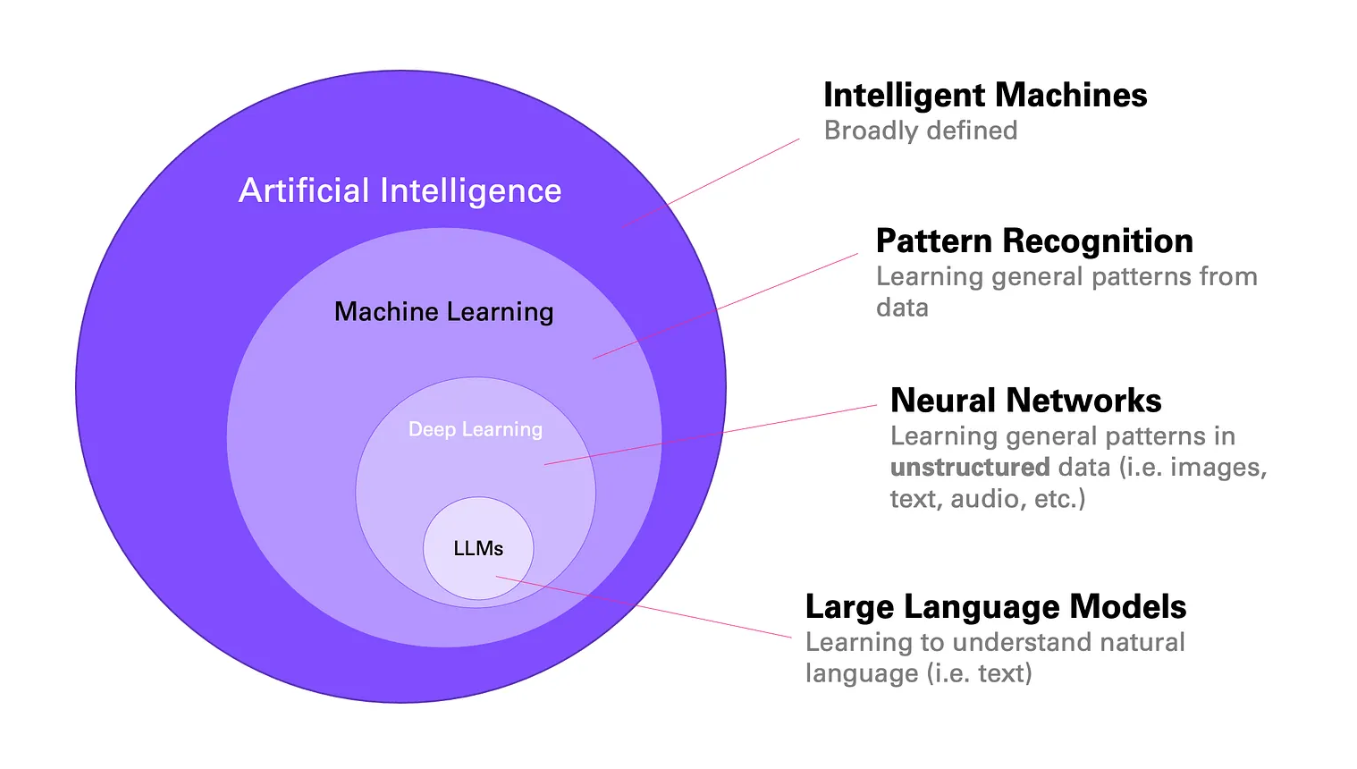
\includegraphics[width=0.5\textwidth]{LLMsphere.png}
  \caption{Artificiële intelligentie in lagen \autocite{Stoeffelbauer2023}}
  \label{fig:LLM-position}
\end{figure}

AI is een brede term, hiermee wordt vaak verwezen naar slimme machines. 
Machine Learning (ML) is een subveld van AI, waarin patronen worden herkend tussen een input en een output.
ML kan gebruikt worden voor verschillende taken zoals: classificatie, regressie, clustering, ... .
Deep Learning (DL) is een subveld van ML, waarin complexe algoritmen en deep neural networks gebruikt worden om moeilijkere taken uit te voeren.
Deep Learning is een krachtige tool die gebruikt wordt voor verschillende taken zoals: beeldherkenning, spraakherkenning, ... \autocite{Stoeffelbauer2023}.

Large Language Modellen zijn geavanceerde AI-systemen die dienen om menselijke taal te verstaan, te genereren en te verwerken.
LLMs worden getraind op een allerlei data zoals artikelen, websites, ... . 
Complexe algoritmen en deep neural networks zorgen ervoor dat LLM's natuurlijke taal verwerken op een gelijkaardige manier zoals een mens dingen verwerkt \autocite{Beelen2023}.
Deze hebben een grote vooruitgang gekend in 2017 door de paper van \textcite{VaswaniEtAl2017}. 
Hieruit kwam een nieuw mechanisme tot stand namelijk transformers wat bestaat uit Attention blokken. 
Het gebruik van deze mechanismen zorgde ervoor dat de LLMs beter presteerden op verschillende taken zoals: vertalen, samenvatten, vragen beantwoorden en tekst genereren.

\subsection{Transformers en de architectuur van LLMs}
\label{sec:architectuur-van-llms}
Een neuraal netwerk bestaat uit verschillende lagen. Enkele belangrijke lagen die gebruikt worden sinds de opkomst van transformers zijn:
\begin{itemize}
  \item Self-Attention
  \item Cross-Attention
  \item Masked Self-Attention
\end{itemize}

Deze lagen worden gebruikt in de encoder en decoder van een transformer en stromen voort uit het onderzoek van \textcite{VaswaniEtAl2017}.

Transformers zijn een speciaal type van neurale netwerken die gebruik maken van verschillende attention blokken.
Attention is een mechanisme dat gebruikt wordt om de relaties tussen verschillende delen van de invoersequenties te leren.
Dit mechanisme is geïnspireerd op de werking van het menselijk brein.
Een transformer bestaat uit een encoder en een decoder. Die elk bestaan uit verschillende attention blokken. 
Dit kan gezien worden in figuur \ref{fig:transformer-model}. 

Self-Attention duidt dynamisch gewichten toe aan verschillende elementen binnen de meegegeven sequentie, bijvoorbeeld woorden in een zin.
Dit laat het model toe om zich te concentreren op de meest relevante delen van de invoer, terwijl de invloed van minder cruciale delen wordt verminderd.
De invoersequentie wordt eerst in drie verschillende vectoren omgezet: query, key en value.
De Query vector stelt een specifiek token uit de invoersequentie voor, de Key vector vertegenwoordigt alle tokens en de vector voor Value bevat de feitelijke inhoud die aan elk token is gekoppeld.
De similariteit tussen de Query en de Key vector wordt berekend aan de hand van het inwendig product van de twee vectoren.
Deze similariteit wordt gebruikt om de gewichten te berekenen die aan de Value vector worden toegekend \autocite{VaswaniEtAl2017}.

Masked Self-Attention is een variant van Self-Attention die gebruikt wordt in de decoder van een transformer.
In de decoder wordt er een mask gebruikt om enkel de vorige tokens te zien in de sequentie \autocite{VaswaniEtAl2017}.
Dit vermijdt dat er informatie van de toekomstige tokens gebruikt wordt. 
Zo kan de transformer niet "vals spelen" tijdens het train proces.

Cross-Attention is een variant van Self-Attention die gebruikt wordt in de decoder van een transformer.
Deze laag gebruikt de informatie van de encoder en de vorige Attention laag van de decoder om de uitvoersequenties te genereren.
De query vector is de uitvoer van de vorige Attention/Cross-Attention laag van de decoder en de key en value vector zijn de uitvoer van de encoder \autocite{VaswaniEtAl2017}.
Doordat de Cross-Attention laag informatie van zowel de encoder als decoder krijgt kan het model de relaties tussen de verschillende delen van de invoersequenties leren.
Deze relaties worden dan gebruikt om de uitvoersequenties te genereren.

\begin{figure}[h]
  \centering
  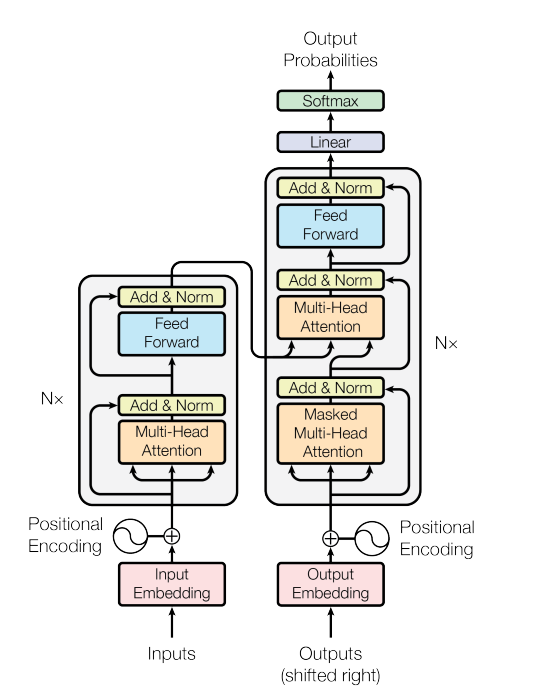
\includegraphics[width=0.5\textwidth]{transformer.png}
  \caption{Transformer - model architectuur \autocite{VaswaniEtAl2017}}
  \label{fig:transformer-model}
\end{figure}

\subsection{Trainen van LLMs}
\label{sec:trainen-van-llms}
Het trainen van LLMs is een complex proces dat veel tijd en rekenkracht vereist. Dit gebeurt in verschillende stappen.
Stap 1 begint bij het verzamelen van een grote hoeveelheid data die gebruikt wordt om het model te trainen.
Deze data kan bestaan uit artikelen, websites, boeken, ... . Zo kan het volgende woord in een sequentie van tekst voorspeld worden.
Deze data wordt gecleaned en geformatteerd zodat het model er mee kan werken.
Uit de data kunnen dan patronen gehaald worden met behulp van Transformers \ref{sec:architectuur-van-llms}, maar het is nog niet instaat om vragen of instructies te begrijpen.

De volgende stap is het model te trainen op een dataset met instructies en het antwoord erop, dit is het gesuperviseerde Fine-Tuning van de LLM \autocite{Das2024}. 
Het model probeert zo de patronen te leren die nodig zijn om vragen te beantwoorden of instructies te volgen.
Dit doet het door de loss te minimaliseren, dit is een maat voor hoe goed het model presteert.
Hierdoor leert het model instructies te volgen en vragen te beantwoorden.

Er kan gebruik gemaakt worden om het model specifiek aan de wensen van de mens te laten voldoen. Dit kan door het gebruiken van Reinfocement Learning met menselijke feedback \autocite{LambertEtAL2022}. 
Hierbij geeft de mens feedback aan het model en leert het model bij door deze feedback.

Het model kan achteraf nog extra getraind worden op specifieke data. 
Het Fine-Tunen van het model kan gebeuren op een specifieke dataset, zoals Python code of medische data.
Dit zorgt ervoor dat het model extra kennis heeft over het gekozen onderwerp.

\subsection{Bestaande LLMs}
\label{sec:bestaande-llms}

Momenteel zijn er verschillende LLMs die gebruikt worden voor verschillende taken.
Deze LLMs zijn getraind op verschillende data en hebben verschillende architecturen.
Het is belangrijk dat er een duidelijk beeld is van de verschillende LLMs en hun mogelijkheden. 
Zodat er een goede keuze gemaakt kan worden voor het genereren van documentatie.

Eén van de grote spelers in de wereld van LLMs is OpenAI. OpenAI heeft verschillende LLMs ontwikkeld gaande van GPT \autocite{RandfordEtAL2018} tot GPT-4 \autocite{OpenAI2023}.
GPT-4 is de krachtigste LLM die OpenAI heeft ontwikkeld, het is getraind op een grote hoeveelheid data en heeft een grote capaciteit.
Een nadeel is dat GPT-4 een betalende service is en niet voor iedereen toegankelijk is \autocite{OpenAI2023}.

Een andere grote speler is Google, Google heeft verschillende LLMs ontwikkeld waaronder BERT van \textcite{DevlinEtAl2019} en Gemini \autocite{Google2024}
BERT staat voor Bidirectional Encoder Representations from Transformers, dit wil zeggen dat het model de context van de woorden kan begrijpen.
BERT was een eerste stap in de wereld van LLMs voor Google. Sinds kort heeft \textcite{Google2024} een nieuwe LLM ontwikkeld genaamd Gemini.
Deze LLM is een sterke concurent voor GPT-4 van \textcite{OpenAI2023}. Het bestaat uit verschillende versies: Gemini Pro, Gemini Ultra en Gemini Nano. 
Elke versie is gemaakt voor een specifiek doeleind, zo is Gemini Nano het meest efficiente model voor mobiele toestellen. Gemini Pro is dan weer het beste model voor het schalen van allerlei taken.
En Gemini Ultra is het meest capabele en grootste model van Google, dit kan gebruikt worden voor complexe taken.
Een van de voordelen van Gemini is dat er een groot aantal input tokens meegegeven kunnen worden, namelijk 1 miljoen tokens.
Dit is aanzienlijk meer dan de 128 duizend tokens van GPT-4.

Een derde speler in de wereld van LLMs is Meta, Meta heeft verschillende LLMs ontwikkeld onder de naam LLama 2 \autocite{Meta2024}.
De LLama 2 familie bestaat uit verschillende LLMs die getraind zijn op verschillende data. Sommige zijn extra getraind voor specifiekere doeleinden.
Zo is er bijvoorbeeld een LLM getraind op Python code, genaamd Code LLama 2 van \textcite{Roziere2024}.
Een voordeel van de LLama 2 familie is dat deze LLMs open source zijn en dus voor iedereen toegankelijk zijn.

Antropic heeft ook een LLM ontwikkeld genaamd Claude \autocite{Antropic2023}. 
Claude's capaciteiten zijn code generatie, het verstaan van meerdere talen, beelden analyseren en kan geavanceerde redeneringen geven.
Er bestaan 3 versies van Claude: Haiku, Sonnet en Opus.
Haiku een lichte versie van Claude, Sonnet is de combinatie van performantie en snelheid en Opus is het intelligentste model dat complexe taken kan uitvoeren en begrijpen.
Claude is een betalende service, de prijzen zijn afhankelijk van de gekozen versie van Claude.

De verschillen tussen deze LLMs zijn groot, zo is er een verschil in capaciteit, trainingsdata en toegankelijkheid.
Het is belangrijk dat er een goede keuze gemaakt wordt voor het genereren van documentatie.
Deze keuze zal afhangen van de mogelijkheden van de LLMs en de doeleinden van de documentatie.
Het is mogelijk dat er meerdere LLMs getest moeten worden om de beste keuze te maken.

\section{Bestaande documentatie tools}
\label{sec:huidige-tools}
Voor er gekeken wordt naar hoe LLMs mogelijk gebruikt kunnen worden voor het genereren van documentatie is het belangrijk dat er een duidelijk beeld is van de huidige tools die gebruikt worden voor het genereren van documentatie.
De documentatie kan in verschillende vormen gegeneerd worden dit kan gaan van een website tot een samenvattend document.
Ook kunnen er in de code zelf commentaren geplaatst worden die de werking van de code uitleggen.
Hiervoor bestaan er reeds verschillende tools en dit voor verschillende programmeertalentalen.

In de paper van \textcite{SridharaEtAL2010} werd er een tool ontwikkel die natuurlijke taal genereert op basis van JAVA code. 
Het selecteert eerst de relevante code en genereert dan een samenvatting van de code, volgens enkele programmeurs die de tool getest hebben was de samenvatting correct en volledig.

Doxygen \autocite{Doxygen2023} is een tool die het toelaat om automatisch code documentatie te genereren. Het is een gratis tool die bruikbaar is voor verschillende programmeertalen zoals: C++, C, Python, PHP en Java.
Het genereert documentatie in de vorm van HTML, LaTeX, RT. Ook is het in staat om een diagram te genereren met de relaties tussen de verschillende delen van de code.
Zo wordt er een duidelijk beeld verkregen van de structuur van het project.

Docstrings is een vorm van commentaar in de code die gebruikt wordt om de werking van de code uit te leggen.
Deze commentaren worden gebruikt om de werking van een module, functie, klasse of methode uit te leggen.
Dit kan automatisch gegenereerd worden met tools zoals CodeCat \autocite{CodeCat2024} voor JavaScript of met de tool van \textcite{Trofficus2023} voor Python.

De tool van \textcite{Trofficus2023} maakt gebruik van GPT-4 \autocite{OpenAI2023} om de docstrings te genereren.
\textcit{Sphinx2023} is een van de meest gebruikte tools voor het genereren van documentatie voor Python projecten.
Het genereert documentatie aan de hand van docstrings en de hierarchie van het project om een duidelijk overzicht te geven.
Deze tool is vrij flexibel want het kan uitgebreid worden met verschillende extensies, zodat het alle mogelijke wensen kan vervullen.

Pdoc \autocite{GallantHils2023} genereert documentatie in de vorm van een website die een API van de documentatie bevat. 
Hier kan er makkelijk op de website gezocht worden naar een functie of klasse met de bijhorende documentatie.

\section{LLM voor documentatie}
\label{sec:llm-voor-documentatie}

Nu er geweten is hoe een LLM werkt en wat het doet. Wat enkele bekende LLMs zijn en wat hun mogelijkheden zijn. 
En wat enkele bestaande documentatie tools zijn.
Is het belangrijk om te kijken naar hoe LLMs gebruikt kunnen worden voor het genereren van documentatie.
Dit kan staps gewijs gebeuren, eerst kunnen de verschillende delen van het project meegegeven worden aan de LLM. 
Hier kan er telkens aan de Large Language Model gevraagd worden om een samenvatting te maken van wat dit deel van het project doet en wat de uitkomst is.
Door dit te herhalen voor alle files van het project kan er achteraf één samenvattend document gemaakt worden van het gehele project.

Ook kan er gevraagd worden aan de LLM om de relatie tussen de verschillende delen van het project te beschrijven in de samenvattingen.
Zo kan er een duidelijk beeld verkregen worden van de structuur van het project en hoe de verschillende delen van het project samenwerken.
Alle functies van het python project kunnen hier makkelijk teruggevonden worden.

Er kan ook gebruik gemaakt worden van de LLM om de docstrings van de verschillende functies en klassen te genereren. 
Om zo een betere samenvatting te verkrijgen van de werking van de verschillende delen van het project, door de docstrings te combineren met de samenvattingen van de LLM.

Wanneer dat een huidige LLM niet instaat is om de gewenste documentatie te genereren kan een LLM gefinetuned op specifieke data, Python code en de bijhorende documentatie.
Hier is er een grote hoeveelheid data van Python projecten met de bijhorende documentatie nodig. Ook is het duur en tijdrovend om een LLM te finetunen.